%% !TeX program = xelatex
%% 부득이하게 pdflatex을 사용해야 할 경우 위의 magic comment를 제거하십시오.

%%%%%%%%%%%%%%%%%%%%%%%%%%%%%%%%%%%%%%%%%%%%%%%%%%%%%%%%%%%%%%%%%%%%%%%%%%%%%%%%%
%%%  LaTeX document class of the thesis of the Gyeonggi Science High School   %%%
%%%  Last edition 2015.11.13 by Chinook Mok                                   %%%
%%%  Continously being modified by gshslatexintro after 2016.02.02.           %%%
%%%  Check the latest version at : latex.gs.hs.kr                             %%%
%%%  Also refer to https://www.facebook.com/gshstexsociety                    %%%
%%%%%%%%%%%%%%%%%%%%%%%%%%%%%%%%%%%%%%%%%%%%%%%%%%%%%%%%%%%%%%%%%%%%%%%%%%%%%%%%%

\documentclass{gshs_thesis}
\graphicspath{{images/}}
% 이곳에 필요한 별도의 패키지들을 적어넣으시오.
%\usepackage{...}
\usepackage{verbatim} % for commment, verbatim environment
\usepackage{spverbatim} % automatic linebreak verbatim environment
%\usepacakge{indentfirst}
\usepackage{tikz}
\usepackage{pgfplots}
%\tikzset{
%	image label/.style={
%		every node/.style={
			%fill=black,
			%text=white,
%			font=\sffamily\scriptsize,
%			anchor=south west,
%			xshift=0,
%			yshift=0,
%			at={(0,0)}
%		}
%	}
%}
\usepackage{amsmath}
\usepackage{amsfonts}
\usepackage{amssymb}
\usepackage{float}
\usepackage{graphicx}
\usepackage{tabularx}
\usepackage{multirow}
\usepackage{booktabs}
\usepackage{longtable}
\usepackage{gensymb}
%\usepackage{subcaption}
%\usepackage{floatrow}
%\usepackage{pict2e}

\usepackage{pgfplots}
\pgfplotsset{
	compat=newest,
	label style={font=\sffamily\scriptsize},
	ticklabel style={font=\sffamily\scriptsize},
	legend style={font=\sffamily\tiny},
	major tick length=0.1cm,
	minor tick length=0.05cm,
	every x tick/.style={black},
}

\usetikzlibrary{shapes}
\usetikzlibrary{plotmarks}
\usepackage{listings}
\usepackage{hologo}
\usepackage{makecell}

\lstset{
	basicstyle=\small\ttfamily,
	columns=flexible,
	breaklines=true
}

\citation
\bibdata



% -----------------------------------------------------------------------
%                   이 부분은 수정하지 마시오.
% -----------------------------------------------------------------------
\titleheader{졸업논문청구논문}
\school{과학영재학교 경기과학고등학교}
\approval{위 논문은 과학영재학교 경기과학고등학교 졸업논문으로\\
졸업논문심사위원회에서 심사 통과하였음.}
\chairperson{심사위원장}
\examiner{심사위원}
\apprvsign{(인)}
\korabstract{초 록}
\koracknowledgement{감사의 글}
\korresearches{연 구 활 동}

%: ----------------------------------------------------------------------
%:                  논문 제목과 저자 이름을 입력하시오
% ----------------------------------------------------------------------
\title{PDMS stamping 방식으로 만든 $\rm{CsPbBr_3}$의 TRPL 분석} %한글 제목
\engtitle{The TRPL analysis of $\rm{CsPbBr_3}$ made with PDMS stamping method} %영문 제목
\korname{김 신 유} %저자 이름을 한글로 입력하시오 (글자 사이 띄어쓰기)
\engname{Kim, Shin You} %저자 이름을 영어로 입력하시오 (family name, personal name)
\chnname{金 信 裕} %저자 이름을 한자로 입력하시오 (글자 사이 띄어쓰기)
\studid{17021} %학번을 입력하시오

%------------------------------------------------------------------------
%                  심사위원과 논문 승인 날짜를 입력하시오
%------------------------------------------------------------------------
\advisor{Park, Kie Hyun}  %지도교사 영문 이름 (family name, personal name)
\judgeone{정 문 석} %심사위원장
\judgetwo{김 제 흥}   %심사위원1
\judgethree{박 기 현} %심사위원2(지도교사)
\degreeyear{2019}   %졸업 년도
\degreedate{2018}{7}{21} %논문 승인 날짜 양식

%------------------------------------------------------------------------
%                  논문제출 전 체크리스트를 확인하시오
%------------------------------------------------------------------------
\checklisttitle{[논문제출 전 체크리스트]} %수정하지 마시오
\checklistI{1. 이 논문은 내가 직접 연구하고 작성한 것이다.} %수정하지 마시오
% 이 항목이 사실이라면 다음 줄 앞에 "%"기호 삽입, 다다음 줄 앞의 "%"기호 제거하시오
%\checklistmarkI{$\square$}
\checklistmarkI{$\text{\rlap{$\checkmark$}}\square$}
\checklistII{2. 인용한 모든 자료(책, 논문, 인터넷자료 등)의 인용표시를 바르게 하였다.} %수정하지 마시오
% 이 항목이 사실이라면 다음 줄 앞에 "%"기호 삽입, 다다음 줄 앞의 "%"기호 제거하시오
%\checklistmarkII{$\square$}
\checklistmarkII{$\text{\rlap{$\checkmark$}}\square$}
\checklistIII{3. 인용한 자료의 표현이나 내용을 왜곡하지 않았다.} %수정하지마시오
% 이 항목이 사실이라면 다음 줄 앞에 "%"기호 삽입, 다다음 줄 앞의 "%"기호 제거하시오
%\checklistmarkIII{$\square$}
\checklistmarkIII{$\text{\rlap{$\checkmark$}}\square$}
\checklistIV{4. 정확한 출처제시 없이 다른 사람의 글이나 아이디어를 가져오지 않았다.} %수정하지 마시오
% 이 항목이 사실이라면 다음 줄 앞에 "%"기호 삽입, 다다음 줄 앞의 "%"기호 제거하시오
%\checklistmarkIV{$\square$}
\checklistmarkIV{$\text{\rlap{$\checkmark$}}\square$}
\checklistV{5. 논문 작성 중 도표나 데이터를 조작(위조 혹은 변조)하지 않았다.} %수정하지 마시오
% 이 항목이 사실이라면 다음 줄 앞에 "%"기호 삽입, 다다음 줄 앞의 "%"기호 제거하시오
%\checklistmarkV{$\square$}
\checklistmarkV{$\text{\rlap{$\checkmark$}}\square$}
\checklistVI{6. 다른 친구와 같은 내용의 논문을 제출하지 않았다.} %수정하지 마시오
% 이 항목이 사실이라면 다음 줄 앞에 "%"기호 삽입, 다다음 줄 앞의 "%"기호 제거하시오
%\checklistmarkVI{$\square$}
\checklistmarkVI{$\text{\rlap{$\checkmark$}}\square$} % usepackage 등의 명령어는 여기에.
\usepackage{cite}
\usepackage{textcomp}
\usepackage{tocloft}
\usepackage{siunitx}
\setlength{\cftbeforesecskip}{0pt}
\setlength{\cftbeforesubsecskip}{0pt}
\setlength{\cftbeforesubsubsecskip}{0pt}

\begin{document}
%	\renewcommand\baselinestretch{1.2} % line spacing in the paragraph

	\baselineskip=2.2em         % line spacing in the paragraph
	\maketitle  % command to print the title page with above variables
\setcounter{page}{1}
%---------------------------------------------------------------------
%                  영문 초록을 입력하시오
%---------------------------------------------------------------------
\begin{abstracts}     %this creates the heading for the abstract page
	\addcontentsline{toc}{section}{Abstract}  %%% TOC에 표시
	\noindent{
		Perovskite is being spotlighted because of its high carrier mobility and cheap price. Also, many new method of making perovskite is being developed rapidly. The aim of this study is to check the capability of PDMS stamping method on making perovskite.
		$\rm{CsPbBr_3}$ solution was spin-coated on the silicon wafer, and was stamped with PDMS to create $\rm{CsPbBr_3}$ single crystal. The crystal structure was checked by X-ray diffraction(XRD) measurement, and its carrier mobility was checked by TRPL measurements. Time resolved photoluminescence(TRPL) measurements showed a consistent ratio between exciton recombination rate and biexciton recombination rate. It ensured that PDMS stamping method was capable of making perovskites. Furthermore, the variation of TRPL data indicates that there is a possibility of calculating the purity quantitatively of the crystal from TRPL datas. 
		\\Key words: TRPL, $\rm{CsPbBr_3}$ single crystal, carrier lifetime
		
	}
\end{abstracts}

\begin{abstractskor}
	페로브스카이트는 전하 수송 능력이 좋고 제조하기 쉽고 값싸다는 데에 장점을 두며 많은 광학 소자에서 응용되고 있다. 특히 이 물질은  태양전지에서 태양에너지를 이용해서 전하를 수송하는 역할로 쓰인다. 
	본 연구에서는 대표적인 페로브스카이트인 $\rm{CsPbBr_3}$  단결정을 비교적 최근에 발견된 방법인 PDMS-stamping 방법으로 만들고, 만들어진 결정이 $\rm{CsPbBr_3}$의 특성을 지니는지 확인한다. X-Ray diffraction (XRD) 을 통해 결정의 구조를 확인하고, Time-Resolved 
	Photoluminescence (TRPL) 분석을 통해 결정의 carrier dynamics를 확인할 수 있다. 이를 기존의 박막 형태의 $\rm{CsPbBr_3}$의 데이터와 이를 비교하였다.  이를 통해 PDMS-stamping 방식이 페로브스카이트를 만드는데 쓰일 수 있다는 것을 보일 수 있으며, 더 나아가 결정의 내부와 외부에서의 TRPL 데이터의 변화를 통해 결정의 순도에 대한 정성적인 예측을 할 수 있다.
	\\Key words: TRPL, $\rm{CsPbBr_3}$ single crystal, carrier lifetime
\end{abstractskor}
%----------------------------------------------
%   Table of Contents (자동 작성됨)
%----------------------------------------------
\cleardoublepage
\addcontentsline{toc}{section}{Contents}
\setcounter{secnumdepth}{3} % organisational level that receives a numbers
\setcounter{tocdepth}{3}    % print table of contents for level 3
\baselineskip=2.2em
\tableofcontents


%----------------------------------------------
%     List of Figures/Tables (자동 작성됨)
%----------------------------------------------
\cleardoublepage
\clearpage
\listoffigures	% 그림 목록과 캡션을 출력한다. 만약 논문에 그림이 없다면 이 줄의 맨 앞에 %기호를 넣어서 코멘트 처리한다.

%\cleardoublepage
%\clearpage
%\listoftables  % 표 목록과 캡션을 출력한다. 만약 논문에 표가 없다면 이 줄의 맨 앞에 %기호를 넣어서 코멘트 처리한다.

%%%%%%%%%%%%%%%%%%%%%%%%%%%%%%%%%%%%%%%%%%%%%%%%%%%%%%%%%%%
%%%% Main Document %%%%%%%%%%%%%%%%%%%%%%%%%%%%%%%%%%%%%%%%
%%%%%%%%%%%%%%%%%%%%%%%%%%%%%%%%%%%%%%%%%%%%%%%%%%%%%%%%%%%
\cleardoublepage
\clearpage
\renewcommand{\thepage}{\arabic{page}}
\setcounter{page}{1}
 % Abstract

	%%%%%%%%%%%%%%%%%%%%%%%%%%%%%%%%%%%%%%%%%%%%%%%%%%%%%%%%%%%
	%%%% Main Document %%%%%%%%%%%%%%%%%%%%%%%%%%%%%%%%%%%%%%%%
	%%%%%%%%%%%%%%%%%%%%%%%%%%%%%%%%%%%%%%%%%%%%%%%%%%%%%%%%%%%
	% Next Section (e.g. Experiment, Linear theory, etc...) 
	% 이외에도 추가로 section마다 파일을 sub 폴더 안에 넣고 여기에서 
	% include 해주면 됩니다.
	% 예시 : methodology.tex을 sub 폴더안에 저장, 이 자리에 
	% \section{실험 과정}

\subsection{준비}
CsPbBr3 용액은 실온 1기압 상태에서 제작되었다. CsPbBr3의 용액을 만들기 위해서 CsBr과 PbBr2를 1:1의 몰 비율로 CsBr 0.638g과 PbBr2 1.101g을 섞었으며 용매인 Dimethyl Sulfoxide (DMSO) 6ml에 섞었다. 용매와 용질을 균일하게 섞기 위해서 50ml들이 통에 담은 후 뚜껑 부분을 파라필름으로 밀봉하고, 통을 물이 담긴 비커에 담은 후 초음파를 이용한 Sonication을 3분간 진행하였다. 

또, Sonication으로 세척한 Silicon wafer 위에 O2 plasma를 이용하여 코팅한 후 3000rpm으로 40초간 spin coating을 이용하여 용액을 균일하게 펼쳐주었다. 마지막으로 미리 100도로 달궈놓았던 핫플레이트에서 5분간 PDMS를 이용하여 눌러주었다. PDMS위에 200g의 무게를 올려놓아 stamping이 잘 일어나도록 하였다. 

\subsection{분석}
CsPbBr3 결정이 만들어졌는지 광학현미경으로 확인한 후, X선 회절법과 TRPL 분석을 진행하였다. XRD measurement는 BRUKER사의 SmartLab 모델을 이용하였고, 입사각을 10°에서 70°까지 변화시키면서 측정하였다. 또, PL과 TRPL는 NT-MDT II Ntegra Spectra DUO Max라는 모델을 이용하여 측정을 하였다. 각각 ND0,ND1필터를 이용해서 측정하였다.
 와 같이 작성
	%%%% 주의
	%%%% 파일이 나뉠 때마다 자동으로 페이지넘김(\clearpage)가 됩니다. 
	%%%% 따라서 subsection을 나누는 용도로는 사용하지 마십시오.
	%%%% \include{sub/experiment} 와 같이...
	
	%-----------------------------------------------------
%  Introduction
%-----------------------------------------------------

\section{서론}

페로브스카이트는 태양 전지에서 빛을 흡수해서 움직이는 전하를 만드는 역할을 한다. 태양 전지가 1970년대 재생 가능 에너지의 일부로써 주목을 받은 이후 지속적인 투자를 받아왔으며 2030년이 되기 전에 광전지로 만드는 전기의 양이 전체 전력의 3분의 1이나 될 것이라는 예측도 있다 \cite{turner2013global}.

\begin{figure}[h!]
	\begin{center}
		\begin{tabular}{cc}
			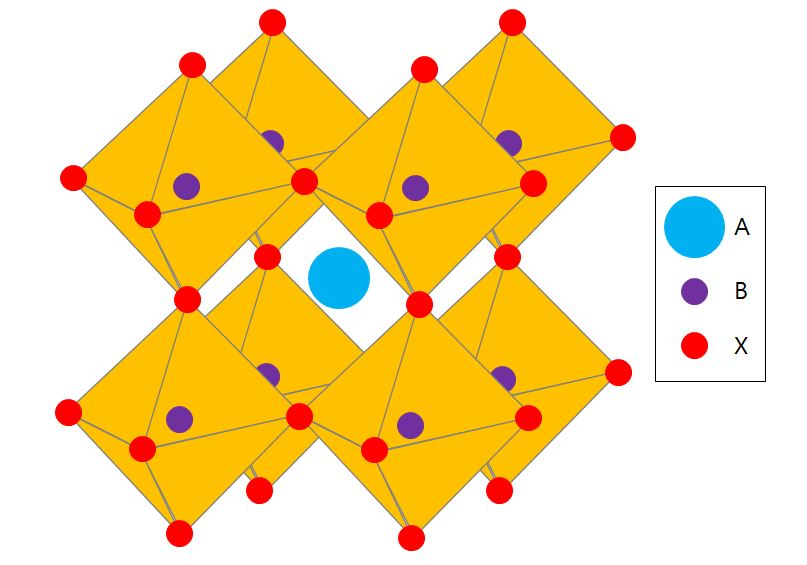
\includegraphics[width=7cm]{perovskite_structure(2)} 
		\end{tabular}
		\caption{The structure of standard perovskite,The octahedral structure on the corner can be seen, made with X. A is a large cation, B is a small cation, and X is the anion, usually hallide and oxide elements.}	
		\label{fig:FIR101}
	\end{center}
\end{figure}

페로브스카이트 재료(이 논문에서 페로브스카이트라고 한다)는 $\rm{ABX_3}$의 결정 구조를 가진 물질로, 여기서 $\rm{A}$, $\rm{B}$는 양이온, X는 음이온이다. 페로브스카이트는 태양전지에서 빛을 받고 원자가 띠에 있는 전자들을 제공하는 역할을 한다. 쇼클리-퀴서 한계(Shockley-Quiesser limit) 이론에 의하면, 하나의 p-n 접합에서 1.34eV의 밴드갭이 형성될 때 에너지 전환 효율이 가장 높은 33.7 \%가 된다고 한다 \cite{ruhle2016tabulated}. 여기서 페로브스카이트의 장점이 대두되는데, A, B, X의 각 구성요소는 상당히 자유롭게 교체할 수 있기 때문에 밴드 간극이  다양한 페로브스카이트가 만들어질 수 있다. 즉, 구성요소를 교체해 밴드갭을 잘 조절하면 이론적으로 최대 효율에 도달하는 페로브스카이트를 만들 수 있다는 의미이다. 또한, 페로브스카이트는 꼭짓점을 공유하는 팔면체 구조를 가지고 있기 때문에 전하 유동성이 뛰어나다\cite{linaburg2015studies}. 이 특성은 페로브스카이트가 빛을 잘 흡수하고 긴 양공 확산 길이를 가질 수 있게 한다\cite{green2014emergence}. 또, 페로브스카이트 태양전지는 전통적인 실리콘 태양전지에 비해 쉽게 만들 수 있다. 페로브스카이트 재료는 100 °C 이하의 온도에서 합성할 수 있는 반면 실리콘 태양전지는 불순물을 제거하기 위해 900 °C 이상의 온도가 필요하다.
많은 연구자들과 과학자들은 이러한 장점을 가진 페로브스카이트를 연구하여, 제조 시간을 줄이고 에너지 전환 효율성을 높이기 위해 활발히 연구하고 있다.

처음으로 페로브스카이트를 이용하여 광 발전을 시도한 사람은 Tsutomu Miyasaka로 2006년에 처음으로 $\rm{CH_3NH_3PbBr_3}$를 이용한 전지로 2.2\%의 효율을 가지는 전지를 만들어 내었다\cite{kojima2006novel}. 2009년에는 Br을 I로 치환하여 효율을 3.8\%까지 올렸다\cite{kojima2009organometal}. 연구는 계속되어 2012년 중반 Henry J.Snaith가  $\rm{CH_{3}NH_3PbI_{3-x}Cl_x}$와 같이 17족 원소들을 섞어서 만드는 페로브스카이트가 안정성과 전하 수송 면에서 우수하다는 것을 보였다\cite{lee2012efficient}. 이후 Seok은 poly-triarylamine을 $\rm{CH_{3}NH_3PbI_{3-x}Br_x}$와 함께 이용하여 12.3\%의 효율을 만들었다\cite{noh2013chemical}.

최근에는 PDMS(Polydimethylsiloxane)를 이용해 단결정 할라이드(hallide) 페로브스카이트를 만드는 새로운 방법이 발견되었다. PDMS는 용액이 웨이퍼에 코팅된 후 압력으로 이를 누르는 데 사용된다. Khoram(2016)은 PDMS stamping으로 만든 $\rm{CsPbBr_3}$의 거칠기가  AFM(Atomic Force Microscopy)으로 측정하였을때 79.1 ± 43.3nm에서 7.1 ± 4.6nm 로 감소했다는 사실을 발견하였다\cite{khoram2016growth}. 또한, 이 방법은 용액에서 석출하는 방법 같은 기존의 방법보다 많은 시간을 절약했다. PDMS stamp를 적용한 연구에서, 할로겐화 페로브스카이트 필름에 약 130nm 크기의 패턴을 성공적으로 인쇄했다\cite{brittman2017controlling}. 이러한 패턴은 1차원 및 2차원 분산 피드백(DFB) 구조에서 표면 반사율을 감소시켜 효율성을 향상시키기 위해 사용될 수 있다.

앞선 논문들에서는 PDMS stamping 방식으로 페로브스카이트를 만들긴 했지만 결정의 특성에 대한 의문을 제기하진 않았다. 새롭게 발견된 방법으로 만들어진 페로브스카이트가 기존의 방법으로 만들어진 페로브스카이트와 같은 특성을 가지고 있다는 것을 증명해야 한다. 그렇기 때문에 이 논문에서는 다음 두 가지 질문에 대해 답하려고 한다.

\begin{enumerate}
	\item PDMS stamping 방법으로 만들어진 단결정 페로브스카이트가 기존의 페로브스카이트와 같은 X선 회절 무늬를 가지고 있는가?
	\item PDMS stamping 방법으로 만들어진 단결정 페로브스카이트의 각 carrier lifetime이 어떻게 변화하는가?
\end{enumerate}

이 문제에 답함으로써 stamped Perovskite의 효율 변화를 규명하고, 추후 연구의 가이드 라인이 될 것으로 보여진다. 이 논문에서는 이를 증명하기 위해 페로브스카이트의 특성을 분석할때에 주로 이용되는 XRD 무늬와 Time-resolved photoluminescence(TRPL) 분석을 이용하였다.

XRD(X-Ray Diffraction)은 결정성 물질에 X선을 쏘아 나타나는 고유 무늬로 물질을 구분하는 것이다. 측정기의 각도를 바꿔가며 도달하는 X선의 세기를 측정하여 무늬를 알아낸다. 

PL(Photoluminescence)은 물질에 에너지를 가해서 들뜬 상태를 만든 후 물질에서 방출되는 빛을 파장별로 검출하는 방식이다. TRPL은 전하 운반자의 시간에 따른 변화를 관찰할 수 있는 장치이다. 이는 PL spectra의 시간에 따른 변화를 확인하는 방식으로, 광발광 수명(photoluminescent lifetime)으로 물질을 식별하거나 LED의 효율을 측정되는 데에 쓰인다. 물질마다 TRPL 데이터의 모양이 다른데, 이는 광발광 수명이 물질의 특성이기 때문이다. $\rm{CsPbBr_3}$의 경우에는 PL의 시간에 따른 변화가 exciton과 biexciton의 재결합에 의해 일어나는데, $\rm{CsPbBr_3}$ 박막에서 각각의 수명은 $\rm{1170~\pm~10~ps}$와 $\rm{510~\pm~5~ps}$ 이다\cite{chen2018room}. 추가하자면, 애초에 TRPL은 carrier dynamics와 lifetime을 가지고 물질이 어떤 식으로 활용될 수 있는지를 예상하는데에 주로 쓰이기 때문에 TRPL 분석으로 보존량을 찾아 물질을 확인하려는 시도는 새로운 것이다. 

이렇게 본 논문에서는 XRD와 TRPL 분석 방법을 이용하여 PDMS stamping을 이용한 새로운 방법이 페로브스카이트를 합성할 수 있다는 것을 보인다.

 % Introduction
	\section{실험 과정}

\subsection{준비}
CsPbBr3 용액은 실온 1기압 상태에서 제작되었다. CsPbBr3의 용액을 만들기 위해서 CsBr과 PbBr2를 1:1의 몰 비율로 CsBr 0.638g과 PbBr2 1.101g을 섞었으며 용매인 Dimethyl Sulfoxide (DMSO) 6ml에 섞었다. 용매와 용질을 균일하게 섞기 위해서 50ml들이 통에 담은 후 뚜껑 부분을 파라필름으로 밀봉하고, 통을 물이 담긴 비커에 담은 후 초음파를 이용한 Sonication을 3분간 진행하였다. 

또, Sonication으로 세척한 Silicon wafer 위에 O2 plasma를 이용하여 코팅한 후 3000rpm으로 40초간 spin coating을 이용하여 용액을 균일하게 펼쳐주었다. 마지막으로 미리 100도로 달궈놓았던 핫플레이트에서 5분간 PDMS를 이용하여 눌러주었다. PDMS위에 200g의 무게를 올려놓아 stamping이 잘 일어나도록 하였다. 

\subsection{분석}
CsPbBr3 결정이 만들어졌는지 광학현미경으로 확인한 후, X선 회절법과 TRPL 분석을 진행하였다. XRD measurement는 BRUKER사의 SmartLab 모델을 이용하였고, 입사각을 10°에서 70°까지 변화시키면서 측정하였다. 또, PL과 TRPL는 NT-MDT II Ntegra Spectra DUO Max라는 모델을 이용하여 측정을 하였다. 각각 ND0,ND1필터를 이용해서 측정하였다.
	
	\section{Results}


\subsection{광학 현미경 관찰}
단결정이 만들어졌는지 확인하기 위하여 현미경으로 관측한 결과를 figure \ref{fig:FIR103}의 사진들로 확인할 수 있다.
\begin{figure}[h!]
	\begin{center}
		\begin{tabular}{ccc}
			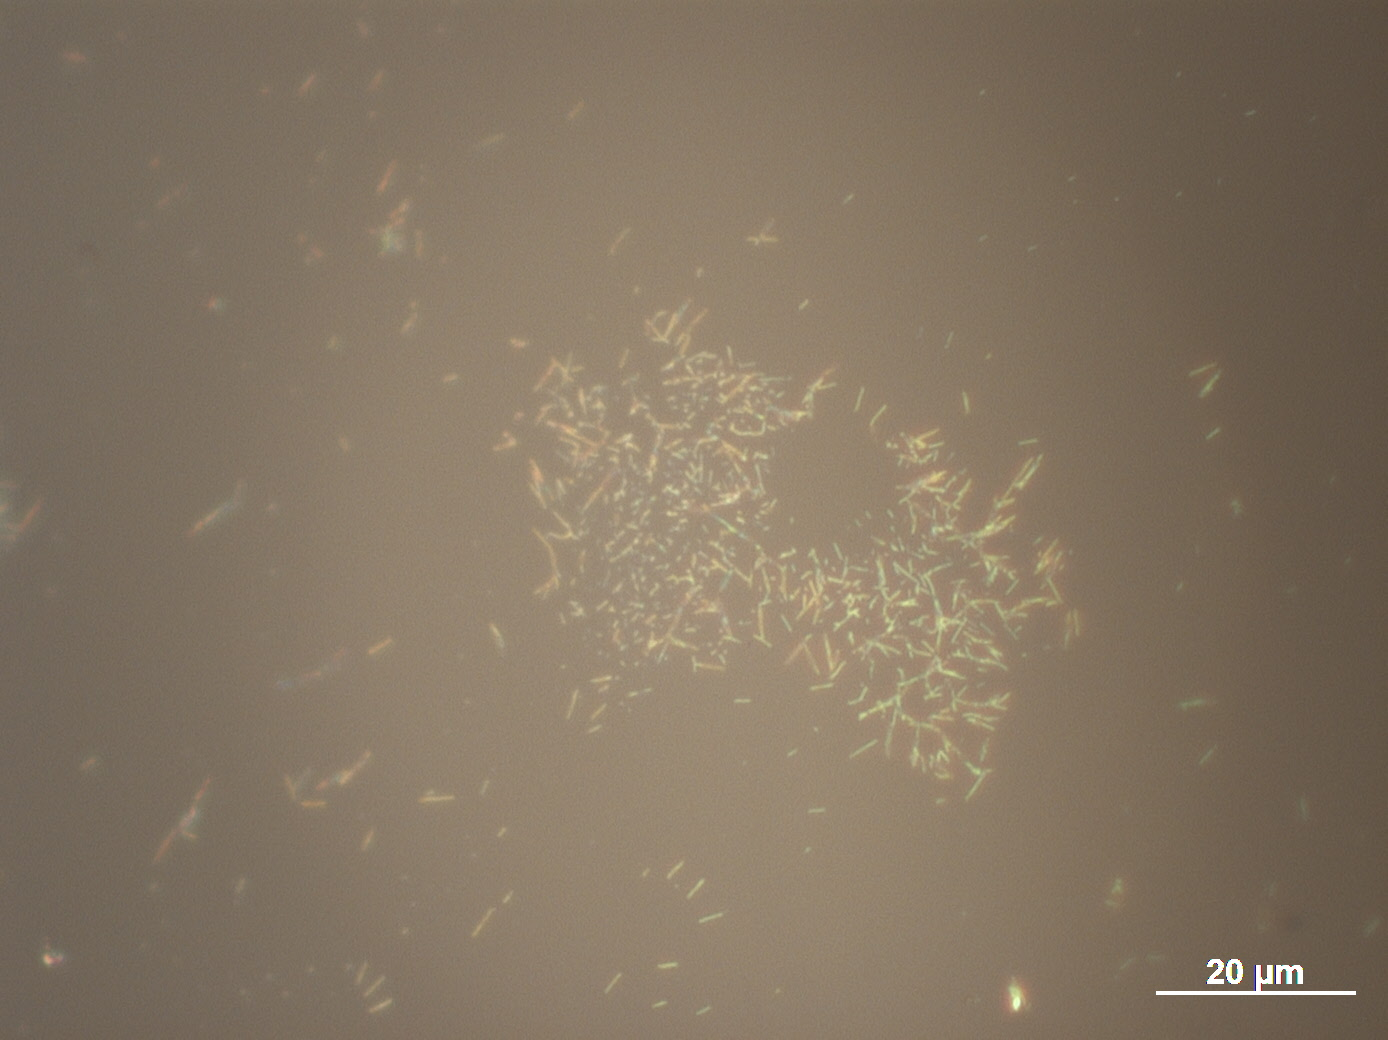
\includegraphics[height=4cm]{optic} &   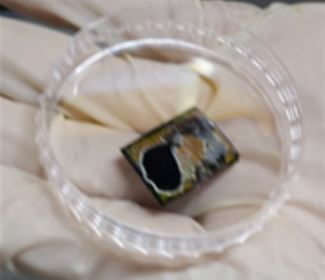
\includegraphics[height=4cm]{crystal}&
			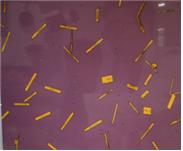
\includegraphics[height=4cm]{crystal_made}
		\end{tabular}
	\begin{tikzpicture} [remember picture,overlay]
	\node[text=white] at (-6.7, 3.8) {(a)};
	\node at (-0.9, 3.8) {(b)};
	\node[text=white] at (4.0, 3.8) {(c)};
	\end{tikzpicture}
		\caption{(a) The picture shows the silicon wafer with no crystals. After the crystal successfully grew, it could be seen by the eyes :(b), and by optic microscopy :(c).}	
		\label{fig:FIR103}
	\end{center}
\end{figure}
\subsection{X-Ray 회절 분석}
$\rm{CsPbBr_3}$의 XRD peak는 2θ = 14.919$^{\circ}$ , 30.099$^{\circ}$ , 47.957$^{\circ}$에서 발견되는 기존의 데이터와 일치하기 때문에 XRD 분석을 통해 $\rm{CsPbBr_3}$ 결정이 만들어졌다는 것을 알 수 있다\cite{rakita2016low}.
\begin{figure}[H]
	\begin{center}
		\begin{tabular}{c}
			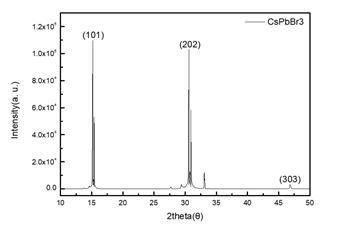
\includegraphics[width=0.50\textwidth]{XRD}
		\end{tabular}
		\caption{The angle of incidence was varied from 10° to 70°. The graph was drawn with Origin 8.0}	
		\label{fig:FIR104}
	\end{center}
\end{figure}


\subsection{TRPL 분석}
TRPL 그래프는 figure \ref{fig:FIR105} 와 같다. t = 28 ns부근에서 최댓값을 확인 할 수 있었고, 그 시간 이후의 데이터를 시간에 따른 지수 함수(exponential function)들의 합으로 fitting 할 수 있는데, 그 식은 $\sum_{i}^{} {e}^{-t/{\tau}_{i}}$ 로 표현된다. $\rm{CsPbBr_3}$는 exciton과 biexciton의 recombination으로 나뉘기 때문에 두 개의 exponential function의 합으로 표현하였다. 그래프의 피팅을 위해 파이썬을 활용하였다. TRPL 데이터를 순서쌍으로 바꿔서 그래프를 그린 후, mathplot library에 내재된 함수인 curve fit을 이용하여 최소제곱법으로 가장 비슷한 함수를 찾아낸다.
\begin{figure}[h]
	\begin{center}
		\begin{tabular}{c}
			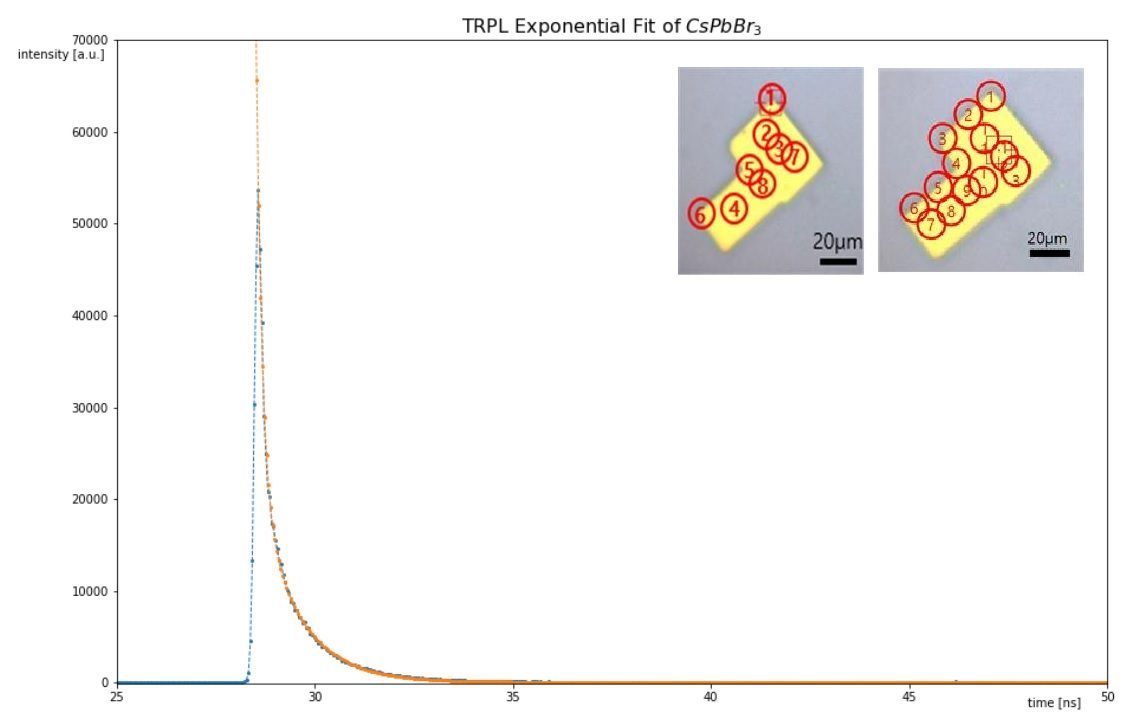
\includegraphics[width=14cm]{TRPL_graph}
		\end{tabular}
		\caption{TRPL graph was fitted with sum of exponential functions.x axis is time(ns) y axis is the intensity of signal(a.u.). Two pictures at the right top shows the point where the TRPL datas were collected. Left picture corresponds to ND0 filter,and the right picture corresponds to ND1 filter. }	
		\label{fig:FIR105}
	\end{center}
\end{figure}
 만들어진 결정이 $\rm{CsPbBr_3}$ 임을 확인하기 위해서 exciton과 biexciton의 recombination rate에 대한 비율을 계산하였다. ND0 필터를 사용했을 때 두 recombination rate 사이의 비율에 대한 평균값은 3.43 이었고 ND1필터를 사용 했을 때는 3.30이었다.
\begin{figure}[t]
	\begin{center}
		\begin{tabular}{cc}
			\begin{tikzpicture}
			\begin{axis} [
			width=0.50\textwidth,%
			height = 6cm,%
			ybar,%
			title={ND0 filter},%
			xtick = data,%
			symbolic x coords={pt1, pt2, pt3, pt4, pt5, pt6, pt7, pt8},%
			ylabel= {ratio},%
			ymin=0,ystep=0.5,ymax=10.0,%
			scaled y ticks = false,%
			ymajorgrids = true,
			legend style={at={(0.02,10)}},legend pos=north west]%
			\addplot table [x=pt, y=data] {./pt_data/ratio_nd0.csv}; %\addlegendentry {2003 LAC}%
			\end{axis}
			\node at (-0.2, 5.0) {(a)};
			\end{tikzpicture}
			&
			\begin{tikzpicture}
			\begin{axis} [
			width=0.50\textwidth,%
			height = 6cm,%
			ybar,%
			title={ND1 filter},%
			xtick = data,%
			symbolic x coords={pt1, pt2, pt3, pt4, pt5, pt6, pt7, pt8, pt9, pt10, pt11},%
			ylabel= {ratio},%
			ymin=0,ystep=0.5,ymax=10.0,%
			scaled y ticks = false,%
			ymajorgrids = true,
			legend style={at={(0.02,10)}},legend pos=north west]%
			\addplot table [x=pt, y=data] {./pt_data/ratio_nd1_2.csv}; %\addlegendentry {2003 LAC}%
			\end{axis}
			\node at (-0.2, 5.0) {(b)};
			\end{tikzpicture}	
		\end{tabular}		
		\caption{The histogram shows the ratio between exciton recombination rate and biexciton rate, differed by the point of laser. (a) is when ND0 filter is used, and (b) is when ND1 filter is used. The standard deviation of ratio is 0.432 and 0.483, respectively. }	
		\label{fig:FIR106}
	\end{center}
\end{figure}
\begin{figure}[h]
	\begin{center}
		\begin{tabular}{ccc}
			\begin{tikzpicture}
			\begin{axis} [
			width=0.5\textwidth,%
			height = 5cm,%
			ybar,%
			bar width=10pt,
			title={ND0 filter},%
			xtick = data,%
			symbolic x coords={pt6, pt4},%
			ylabel= {nsec},%
			ymin=0,ystep=0.2,ymax=2.5,%
			scaled y ticks = false,%
			ymajorgrids = true,
			legend style={at={(0.02,10)}},legend pos=north west]%
			\addplot table [x=pt, y=tau1] {./ND_data/nd0_1.csv}; \addlegendentry {tau 1},%
			\addplot table [x=pt, y=tau2]
			{./ND_data/nd0_1.csv}; \addlegendentry {tau 2}%
			\usetikzlibrary{patterns},
			\end{axis}
			\node at (-0.2, 4.0) {(a)};
			\end{tikzpicture}
			&
			\begin{tikzpicture}
			\begin{axis} [
			width=0.4\textwidth,%
			height = 5cm,%
			ybar,%
			bar width=10pt,
			title={ND0 filter},%
			xtick = data,%
			symbolic x coords={pt1, pt2, pt3},%
			ylabel= {nsec},%
			ymin=0,ystep=0.2,ymax=2.5,%
			scaled y ticks = false,%
			ymajorgrids = true,
			legend style={at={(0.02,10)}},legend pos=north west]%
			\addplot table [x=pt, y=tau1] {./ND_data/nd0_2.csv}; \addlegendentry {tau 1},%
			\addplot table [x=pt, y=tau2]
			{./ND_data/nd0_2.csv}; \addlegendentry {tau 2}%
			\end{axis}
			\node at (-0.2, 4.0) {(b)};
			\end{tikzpicture}
			&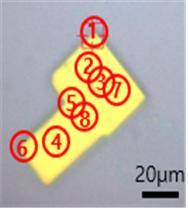
\includegraphics[width=3cm]{nd0place}
			\begin{tikzpicture} [remember picture,overlay]
			\node at (-2.8, 3.0){(c)};
			\end{tikzpicture}
				
		\end{tabular}		
		\caption{Both exciton / biexciton recombination rate increased when the laser point headed to the center of the crystal. The unit of y-axis is ns. ND0 filter is used. Tau 1 means the exciton recombination rate, and tau 2 mean the biexciton recombination rate.}	
		\label{fig:FIR107}
	\end{center}
\end{figure}

Figure 7은 exciton / biexciton recombination rate의 비율이 아닌, 값 자체를 히스토그램으로 나타낸 것으로, 두 값 모두가 결정의 중심쪽으로 갈수록 증가하고 있음을 관찰할 수 있다. (c)는 (a)와 (b)에서의 x축에 해당하는 점들의 위치를 표시하고 있다. (a)의 경우 TRPL 데이터가 점 6에서 점 4로 갈 때에 recombination rate가 증가하는 것을 볼 수 있다. pt 1, 2, 3의 경우에는 pt 3의 exciton recombination rate가 약간 감소하였으나, 그 이상으로 biexciton recombination rate가 증가했기 때문에 감소한 exciton recombination이 biexciton recombination으로 대체되었다고 할 수 있었다.
마찬가지로 (b)의 경우에도 TRPL 데이터가 점 1에서 2를 거쳐 3으로 갈 때에도 recombination rate가 증가하였다.
Figure 8은  Figure 7과 마찬가지로 결정의 중심부분으로 갈수록 recombination rate가 증가하는 모습을 보여준다. 하지만, 이때는 Figure 7과는 다르게 pt 9에서 pt 10으로 향할 때는 두 rate가 모두 감소하였는데, 이는 결정의 중심부에서 결정이 완성되지 못했음을 의미한다. 

\begin{figure}[H]
	\begin{center}
		\begin{tabular}{ccc}
			\begin{tikzpicture}
			\begin{axis} [
			width=0.4\textwidth,%
			height = 5cm,%
			ybar,%
			bar width=10pt,
			title={ND0 filter},%
			xtick = data,%
			symbolic x coords={pt2, pt11, pt12},%
			ylabel= {nsec},%
			ymin=0,ystep=0.2,ymax=2.5,%
			scaled y ticks = false,%
			ymajorgrids = true,
			legend style={at={(0.02,10)}},legend pos=north west]%
			\addplot table [x=pt, y=tau1] {./ND_data/nd1_1.csv}; \addlegendentry {tau 1},%
			\pagestyle{empty}
			\addplot table [x=pt, y=tau2]
			{./ND_data/nd1_1.csv}; \addlegendentry {tau 2}%
			\end{axis}
			\node at (-0.2, 4.0) {(a)};
			\end{tikzpicture}
			&
			\begin{tikzpicture}
			\begin{axis} [
			width=0.4\textwidth,%
			height = 5cm,%
			ybar,%
			bar width=10pt,
			title={ND0 filter},%
			xtick = data,%
			symbolic x coords={pt6, pt7, pt8, pt9, pt10},%
			ylabel= {nsec},%
			ymin=0,ystep=0.2,ymax=2.5,%
			scaled y ticks = false,%
			ymajorgrids = true,
			legend style={at={(0.02,15)}},legend pos=north west]%
			\addplot table [x=pt, y=tau1] {./ND_data/nd1_2.csv}; \addlegendentry {tau 1},%
			\addplot table [x=pt, y=tau2]
			{./ND_data/nd1_2.csv}; \addlegendentry {tau 2}%
			\end{axis}
			\node at (-0.2, 4.0) {(b)};
			\end{tikzpicture} &
			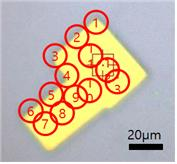
\includegraphics[width=3cm]{nd1place}
			\begin{tikzpicture} [remember picture,overlay]
			\node at (-2.8, 2.5){(c)};
			\end{tikzpicture}
		\end{tabular}
		\caption{Same tendency can also be seen when ND1 filter is used.}	
		\label{fig:FIR109}
	\end{center}
\end{figure} 
	%-----------------------------------------------------
% Conclusion
%-----------------------------------------------------
\newpage

\section{Conclusion}
본 연구의 결과는 다음과 같다:
\begin{enumerate} 
	\item PDMS stamping 방식으로 만들어진 결정은 광학 현미경을 통해 육안으로 확인하였고, X선 회절법을 이용하여 이 결정이 기존의 결정과 같은 X선 회절 무늬를 가지고 있음을 확인 할 수 있었다.
	\item	
	Exciton recombination rate와 biexciton recombination rate 사이의 비율의 평균값은 ND 0 filter 일 때는 3.43, ND 1 filter일 때는 3.30이었다. 이론적으로 알려진 2.29라는 비율\cite{chen2018room} 과는 다소 상이하였으나 두 재결합률 사이의 비율이 결정의 위치가 바뀌어도 일정한 것으로 보아 만들어진 결정이 동일한 특성을 보인 물질이라는 것을 확인 할 수 있었다. 두 값이 약간의 차이를 갖는 이유는 2.29라는 값은 $\rm{CsPbBr_3}$ 박막의 값이지만 3.30 나 3.43이라는 값은 $\rm{CsPbBr_3}$ 단결정의 값이기 때문이라고 예상된다.  
	\item 결정의 중심부로 갈수록 커지는 exciton / biexciton recombination rate로부터 결정의 중심부 결정의 순도가 높아진다는 경향성을 찾을 수 있었다. recombination rate가 커진다는 것은 원자가띠에 인접한 defect의 에너지띠보다 전도띠에서 더 많은 recombination이 일어났다는 의미이다. 그렇기 때문에 recombination rate가 증가하면, defect가 적다는 의미이고, 순도가 높다는 의미이기도 하다.
	\item TRPL 데이터의 분석을 통해 Figure 8의 pt 10은 중심부로 갈수록 오히려 exciton / biexciton recombination rate가 감소하는 양상을 보여주었는데, 이는 중심부로 갈수록 순도가 감소한다는 것을 의미하는 것이 아니라 이 부분의 결정이 불완전하게 생성되었음을 의미한다. 즉, PDMS-stamping의 시간을 연장하거나 온도 조건을 조절함으로써 pt 10의 결정을 완성한다면 예측과 같이 순도가 증가할 것으로 예상된다. 
\end{enumerate}
PDMS-stamping 방법으로 만든 $\rm{CsPbBr_3}$ 단결정이 기존의 $\rm{CsPbBr_3}$와 동일하다는 것은 X선 회절 분석으로 보일 수 있었다. 하지만, TRPL 분석을 통해 보존되는 비율로 만들어진 결정이 $\rm{CsPbBr_3}$임을 보이려는 시도는 성공적이지 못했다. 그렇기 때문에 단결정이 만들어졌다는 결론은 X선 회절 분석으로 내린 후, TRPL 분석 결과로는 exciton recombination rate 와 biexciton recombination rate사이의 비율이 PDMS-stamping 방법으로 만든 단결정이 더 크게 관찰되었기 때문에 이 단결정이 기존의 단결정보다 exciton의 recombination이 활발하게 일어난다는 것을 유추하는 것이 올바른 해석이었다.  
또, 결과 3번 항목에서 결정의 순도의 비교는 오직 정성적으로 이루어졌다. 그렇기 때문에 만약 recombination rate와 결정의 순도 간의 정량적인 관계를 구할 수 있다면 결정의 순도를 유추할 수 있는 획기적인 방법이 될 것이다.
마지막으로 박막 형태의 $\rm{CsPbBr_3}$와 단결정 $\rm{CsPbBr_3}$에서의 exciton recombination rate과 biexciton recombination rate 사이의 비율이 약간의 차이를 갖는 이유에 대해서는 추가적인 실험과 연구가 필요할 것으로 보이고, exciton이 우세한 $\rm{CsPbBr_3}$가 필요한 분야에 대한 탐색이 이루어져야 할 것이다. 


 % Conclusion
	
	%%\clearpage  %%% Appendix를 새 페이지에서 시작
\appendix
\renewcommand{\thesection}{\Alph{section}} %%% TOC에 appendix numbering 재설정
\renewcommand{\thesubsection}{\arabic{subsection}}
\renewcommand{\thesubsubsection}{\arabic{subsubsection}}
\titleformat{\section}[hang] {\normalfont\fontsize{21}{21}\selectfont\bfseries}{\Alph{section}.}{1em}{} %%% Appendix section title의 재설정
\titleformat{\subsection}[hang] {\normalfont\fontsize{16}{16}\selectfont\bfseries}{\Alph{section}.\arabic{subsection}.}{1em}{}
\titleformat{\subsubsection}[hang] {\normalfont\fontsize{14}{14}\selectfont}{\Alph{section}.\arabic{subsection}.\arabic{subsubsection}.}{1em}{}
\titleformat{\paragraph}[hang] {\normalfont\fontsize{12}{12}\selectfont\it}{}{1em}{}
\renewcommand{\theequation}{\thesection.\arabic{equation}} %%% Appendix equation numbering 의 재설정
\renewcommand{\thefigure}{\thesection-\arabic{figure}} %%% Appendix figure numbering 의 재설정
\renewcommand{\thetable}{\thesection-\arabic{table}} %%% Appendix table numbering 의 재설정
\setcounter{equation}{0} %%% Appendix equation starting number의 초기화
\setcounter{figure}{0} %%% Appendix figure starting number의 초기화
\setcounter{table}{0} %%% Appendix table starting number의 초기화
\section{부록}
\begin{table}[h!]
	\begin{center}
		\begin{tabular}{c|c|c|c|c|c|c|c|c}
			\toprule
			&\multicolumn{4}{c|}{Previous Work} & \multicolumn{4}{c}{Our Work}\\
			&\multicolumn{2}{c|}{Blue Lobe} & \multicolumn{2}{c|}{Red Lobe} & \multicolumn{2}{c|}{Blue Lobe} & \multicolumn{2}{c}{Red Lobe}\\
			\textbf{Name} & $\mathbf{v_{out}}$ & $\mathbf{v_{in}}$ & $\mathbf{v_{out}}$ & $\mathbf{v_{in}}$&$\mathbf{v_{out}}$ & $\mathbf{v_{in}}$ & $\mathbf{v_{out}}$ & $\mathbf{v_{in}}$\\
			& [km/s] & [km/s] & [km/s] & [km/s] & [km/s] & [km/s] & [km/s] & [km/s] \\ 
			\midrule
			\multicolumn{9}{c}{Orion A Cloud}\\
			\midrule
			FIR2 & -4.1 & 8.9 & 13.2 & 20.8 &-4.1 & 9.4 & 12.9 & 20.8\\
			FIR3 & -4.1 & 8.9 & 13.2 & 25.1 & -4.1 & 9.25 & 13.0 & 25.1\\
			FIR6b & 1.3 & 8.9 & 13.2 & 21.9 & 1.3 & 9.3 & 12.4 & 21.9\\
			MMS2 & 3.5 & 8.9 & 13.2 & 16.5 & 3.5 & 8.8 & 12.8 & 16.5\\
			MMS5 & 1.3 & 8.9 & 13.2 & 21.9 & 1.3 & 9.5 & 13.1 & 21.9\\
			MMS9 & -4.1 & 8.9 & 13.2 & 26.2 & -4.1 & 9.6 & 13.0 & 26.2\\
			\midrule
			\multicolumn{9}{c}{$\rho$ Ophiuchus Cloud}\\
			\midrule
			Elias 32 & -6.7 & 0.8 & 6.0 & 10.3 & -6.7 & 1.2 & 5.3 & 10.3\\
			IRS 46 & -3.7 & 0.4 & 6.5 & 14.1 & -1.2 & 1.1 & 5.9 & 8.4\\
			VLA 1623 & -3 & 10 & 6.5 & 13 & -3 & 1.2 & 5.3 & 9\\
			BBRCG 24 & N.A. & N.A. & N.A. & N.A. & -5 & 1.2 & 5.7 & 9\\
		\end{tabular}
	\end{center}
	\caption{관측한 원시성들의 적색/청색편이 속도 구간}
\end{table} % Appendix가 없는 경우 주석처리하십시오
	
	\bibliography{bibfile} % 참고문헌
	% BibTeX 코드 쉽게 얻어오는 방법 %
	% Google Scholar 에서 검색한 결과에서 `인용'을 클릭한다.
	% BibTeX 코드를 얻고자 한다면, 하단의 `BibTeX' 을 클릭.
	% 코드가 나온다. Ctrl+A, Ctrl+C로 복사, bibfile에 붙여넣기.
	
	%\begin{summary}
\addcontentsline{toc}{section}{Summary}  %%% TOC에 표시
한글로 졸업논문을 작성한 학생은 반드시 5페이지 내외의 영어 요약문을 작성해야 합니다. 영문으로 작성하는 학생은 이 부분을 작성하지 않아도 됩니다.
\end{summary} % Summary
	%(영어로 작성한 학생은 이 부분을 주석 처리하십시오.)
	
	%-----------------------------------------------------
%   감사의 글
%-----------------------------------------------------

%-----------------------------------------------------
%   연구활동 
%-----------------------------------------------------
%\begin{researches}
%\addcontentsline{toc}{section}{Summary}  %%% TOC에 표시
%\begin{itemize}
%\item{2017학년도 교내 R\&E 발표대회에서 우수상 수상}

%\end{itemize}
%\end{researches} % 감사의 글 & 연구활동
\end{document}